% Research workflow diagram (same TikZ source as Figure 1 of the final report).
% Build: pdflatex workflow_diagram.tex, then pdftoppm -r 250 -png -singlefile workflow_diagram.pdf workflow_diagram
\documentclass[border=8pt]{standalone}
\usepackage{times}
\usepackage{xcolor}
\usepackage{xspace}
\usepackage{tikz}
\usetikzlibrary{positioning,arrows.meta}
\definecolor{cvprblue}{rgb}{0.21,0.49,0.74}
\newcommand{\tabicl}{TabICL\xspace}
\begin{document}
  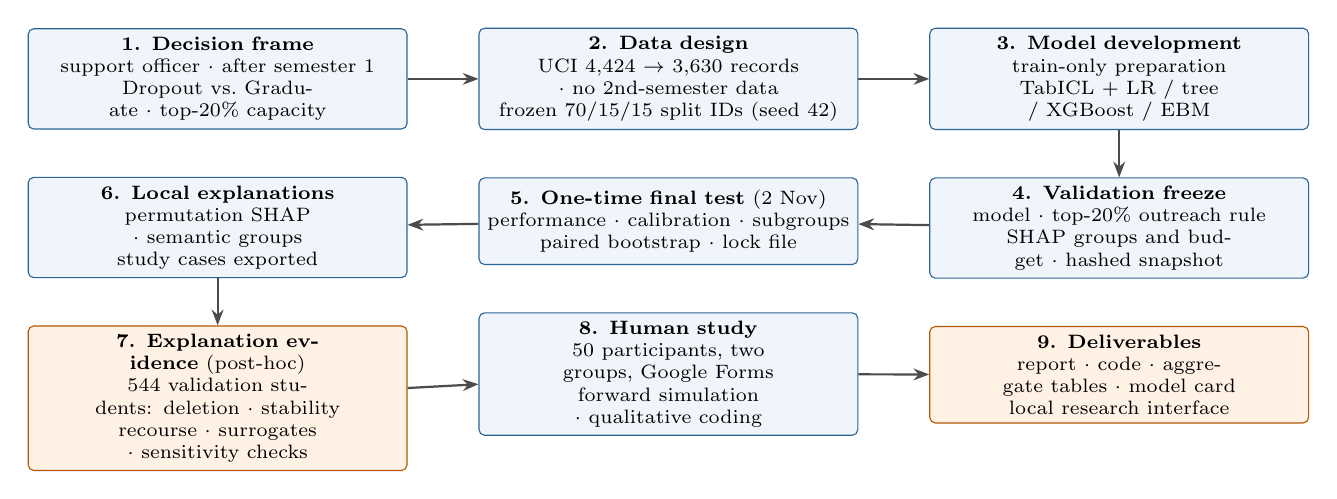
\begin{tikzpicture}[
    node distance=6mm and 9mm,
    box/.style={draw=cvprblue!80!black, fill=cvprblue!8, rounded corners=2pt, align=center,
                font=\scriptsize, minimum height=11mm, text width=4.6cm, inner sep=3pt},
    post/.style={box, fill=orange!10, draw=orange!70!black},
    arr/.style={-{Stealth[length=2mm]}, thick, draw=black!70}]
    % row 1 (left to right)
    \node[box] (n1) {\textbf{1. Decision frame}\\support officer $\cdot$ after semester 1\\Dropout vs.\ Graduate $\cdot$ top-20\% capacity};
    \node[box, right=of n1] (n2) {\textbf{2. Data design}\\UCI 4,424 $\rightarrow$ 3,630 records $\cdot$ no 2nd-semester data\\frozen 70/15/15 split IDs (seed 42)};
    \node[box, right=of n2] (n3) {\textbf{3. Model development}\\train-only preparation\\\tabicl + LR / tree / XGBoost / EBM};
    % row 2 (right to left)
    \node[box, below=of n3] (n4) {\textbf{4. Validation freeze}\\model $\cdot$ top-20\% outreach rule\\SHAP groups and budget $\cdot$ hashed snapshot};
    \node[box, below=of n2] (n5) {\textbf{5. One-time final test} (2 Nov)\\performance $\cdot$ calibration $\cdot$ subgroups\\paired bootstrap $\cdot$ lock file};
    \node[box, below=of n1] (n6) {\textbf{6. Local explanations}\\permutation SHAP $\cdot$ semantic groups\\study cases exported};
    % row 3 (left to right)
    \node[post, below=of n6] (n7) {\textbf{7. Explanation evidence} (post-hoc)\\544 validation students: deletion $\cdot$ stability\\recourse $\cdot$ surrogates $\cdot$ sensitivity checks};
    \node[box, below=of n5] (n8) {\textbf{8. Human study}\\50 participants, two groups, Google Forms\\forward simulation $\cdot$ qualitative coding};
    \node[post, below=of n4] (n9) {\textbf{9. Deliverables}\\report $\cdot$ code $\cdot$ aggregate tables $\cdot$ model card\\local research interface};
    \draw[arr] (n1) -- (n2); \draw[arr] (n2) -- (n3); \draw[arr] (n3) -- (n4);
    \draw[arr] (n4) -- (n5); \draw[arr] (n5) -- (n6); \draw[arr] (n6) -- (n7);
    \draw[arr] (n7) -- (n8); \draw[arr] (n8) -- (n9);
  \end{tikzpicture}
\end{document}
